\documentclass[pdftex,final]{pittetd}
%final, makes pittetd's warnings (about things that might go against the Format Guidelines) into error messages. 
%Option 'sectionletters' numbers the chapters with Roman numerals (I, II, etc.), sections with 
%letters (A, B), subsections with numbers (1, 2), and subsubsections with lowercase letters (a, b). 
%The four levels of the enumerate environment receive the same treatment. Within the
%text, however, cross references (\ref} produce `the whole thing,' something like I.A.1 
%instead of only 1.

% Packages included in PittETD Template
% auto use this package and check for patches
\usewithpatch{graphicx} 
% manually use these packages
\usepackage{amsmath}
% manually check for patches
\patch{amsmath}
%\patch{amsthm}

% Jenna's commonly used packages
\usepackage{amssymb}
\usepackage{amsmath}
%\usepackage{amsthm}
\usepackage{graphics} % for improved inclusion of graphics
%\usepackage{wrapfig} % to include figure with text wrapping around it
%\usepackage{subcaption}
%\usepackage[margin=10pt,font=small,labelfont=bf]{caption}
\usepackage{algorithm}
%\usepackage{algorithmic}
\usepackage{algpseudocode}

% Bibliography
\bibliographystyle{apalike}

\title[Exploring and Correcting Motion in Resting-State Functional Magnetic Resonance Images of Congenital Heart Disease Patients]{Exploring and Correcting Motion in Resting-State Functional Magnetic Resonance Images of Congenital Heart Disease Patients}
% The optional argument is the 
% version of the title that will appear in Acrobat Reader's Document Info dialog box.
\author{Jenna Marie Schabdach}
\degree{B. S. Electrical Engineering, Drexel University, 2016\\M. S. Electrical Engineering, Drexel University, 2016\\M. S. Biomedical Informatics, University of Pittsburgh, 2018}

%\date{July 20th 1967}%             This date is the date of the thesis defense. Default is \today
% pittetd will use the current year unless otherwise indicated. So this command is not necessary.
\keywords{\LaTeX, pittetd, theses, format}% This list appears in the field 'Keywords' of Acrobat Reader's Document Info
%                                   dialog box, and also, optionally, after the abstract.
\subject{Schabdach Biomedical Informatics Dissertation}%              This fills in the 'Subject' field in Acrobat Reader's Document Info dialog box.
\school{Department of Biomedical Informatics}%    The name of the school will be preceeded by 'the' unless otherwise specified, as in:
%\school[certain]{department}

\begin{document}

\year{2019}  
%\chapterfloats%                    Un-comment this to get figures and tables numbered within chapters.
\maketitle
%
% For the committee membership page, you have to provide the names and affiliations of the members. The first one will 
% be treated by pittetd as the committee chair (thesis/dissertation advisor).
\committeemember{Dr. Douglas Landsittal, Department of Biomedical Informatics}
%\coadvisor{Second advisor, Dept. Aff.}%         This is used if there are two advisors.
\committeemember{Dr. Ashok Panigrahy, Department of Biomedical Informatics}
\committeemember{Dr. Gregory Cooper, Department of Biomedical Informatics}
\committeemember{Dr. Rafael Ceschin, Department of Pediatric Radiology, Children's Hospital of Pittsburgh of UPMC}

% etc., as many as needed. For master's theses, the committee may be omitted, naming only the advisor.
\school{School of Medicine}
\makecommittee
%\copyrightpage                     Uncomment this to get a copyright page.
\begin{abstract}
INSERT ABSTRACT HERE
\end{abstract}
% If you say \begin{abstract}[Keywords:] instead of the simple \begin{abstract}, a list of the keywords is appended.
% The list comes from the \keywords command above.
% The starred version \begin{abstract*} typesets the word `ABSTRACT' on the top of the page
\tableofcontents
%\listoftables                      % Pittetd will complain if you tell it to create a list of tables when there are no
%                                   tables (as in this sample file). Uncomment this command if you have tables.
%\listoffigures                     % Obvious analogous for figures.
%\preface
% This is the text of the preface, with acknowledgments, dedication, etc. It is optional, and you create, as shown, by 
% just saying \preface and starting the preface's actual text. Note that 'foreword' is no longer acceptable as title
% for this preliminary.
%
%Conventions, such as notation (nomenclature) and abbreviations, don't receive their own preliminary page. They can be included as an appendix, or as part of the introduction.


% Add in chapters here
\chapter{Introduction}

Resting-state functional magnetic resonance imaging (rs-fMRI) measures the blood oxygen level dependent signal in an organ or organ system. This property makes rs-fMRI an invaluable tool for evaluating a patient's neurodevelopmental status or examining functional networks in his brain. To gather enough data to fully evaluate these networks, a series of image volumes must be acquired over a period of several minutes. In a standard rs-fMRI (?), one new image volume is obtained approximately once every two to three seconds. To gather high quality data on such a short timescale, the rs-fMRI suffers from two major limitations: rs-fMR images have low physical resolution and are highly susceptible to motion. The first limitation can be addressed by obtaining an MR image with high physical resolution and registering the rs-fMRI to this structural image, but the second limitation requires the patient to remain as still as possible for the entire duration of the scan. This task is particularly difficult for populations of certain ages or populations who suffer from conditions that affect neurodevelopment. As a result, it is common for an image from a member of one of these populations to contain too much motion to be used in clinical or research applications.

Various behavioral and XX protocols have been developed in an attempt to prevent patients from moving during MRI scans, though many of these protocols are not applicable to younger populations. In particular, a neonate or fetus cannot understand instructions to stay still, and young children who can understand the command have difficulty following it. Sedation is not advisable for these young populations. After a rs-fMR image is acquired, however, it is possible to reduce the positional effects of motion in the image sequence.

Limitations of traditional methods

DAG-based registration

Apply DAG-based registration to neonates and preadolesents

Real goal is to develop a method of registering fetal brain and placental images so that we can further examine the relationship between placental oxygen levels and fetal brain development. Longitudinally, this technique can be used to determine how placental oxygen flow and fetal brain development impact a patient over the course of his or her life. Once the relationship between the placenta and fetal brain development is better understood, we can determine a set of neuroprotective interventions to employ for at-risk patients before they are born.
\chapter{Neurodevelopment, Congenital Heart Disease, and Functional Connectivity}
\label{ch:clinical}

\section{CONGENITAL HEART DEFECTS}

Congenital heart defects and congenital heart disease (CHD) both refer to defects in the heart or the vessels around the heart which formed during  fetal development. Heart defects affect how blood moves into, through, and away from the heart. 
CHD can affect any combination of heart chambers and blood vessels with varying degrees of severity. The lesions prevent the cardiopulmonary system as a whole from functioning correctly, but pinpointing and treating the defects effectively can be a complex process.
 
% Causes of CHD: genetic syndromes, single gene mutations, environmental exposure, and unknown
There are a number of genetic and environmental factors associated with CHD \cite{Mozaffarian2016}. Genetic conditions such as Down syndrome, Turner syndrome, 22q11 deletion syndrome, Williams syndrome, and Noonan syndrome are associated with different CHD presentations. Maternal behaviors such as smoking and binge drinking are known to cause heart problems in the fetus. Other maternal risk factors are obesity, folate deficiency, and living at a high altitude. Paternal exposure to phthalates, anesthesia, sympathomimetc medications, pesticides, and solvents may increase the risk of the fetus for developing CHD. While there are quite a few factors in this list, there are many CHD cases whose causes are unknown.

\begin{figure}
\centering
\includegraphics[width=0.6\textwidth]{2/chd-defects-usa.png}
\label{ch2:fig:usa-defects-prev}
\caption{Table of prevalences of congenital heart defects borrowed temporarily from \cite{Mozaffarian2016}.}
\end{figure}

% Diagnosis
The process of diagnosing CHD can begin before birth. A specialized ultrasound test called fetal echocardiography can detect heart abnormalities as early as the second trimester of the pregnancy. Additional tests, such as amniocentesis and follow-up ultrasounds may be needed to determine treatment options. Generally, severe CHD cases present and are detected at earlier stages, but minor defects may not become apparent until the patient is older. 
The incidence of CHD in live births vary across countries and continents: the United States reports approximately 4-10 CHD case per 1,000 live births, while Europe and Asia see about 6.9 and 9.3 CHD cases per 1,000 live births \cite{Mozaffarian2016}.
%It is important to note that these incidence rates only report the incidence of CHD as detected at birth, not cases detected later in the patient's life. % Is this correct?
A breakdown of prevalence rates of some of the most common lesion types can be seen in \ref{ch2:fig:usa-defects-prev}.
As screening tools become more effective, it is expected that these rates will increase as defects are detected earlier. % See (16)

Once a patient is diagnosed with one of these defects, the specific nature of his case must be clearly documented. The documentation of CHD using the International Classification of Diseases, Ninth Revision, Clinical Modification (ICD-9-CM) has 25 high level codes representing various presentations of CHD, but these codes used on their own are often not sufficient for describing a patient's true condition \cite{Mozaffarian2016}. Additional ICD-9-CM codes may be used to communicate the finer details of a patient's condition. 

%Depending on the cause of the 

Financial burden: high for certain defects, medium costs for surgical interventions for other lesions, still processing \cite{Mozaffarian2016}

% Complications and risks
Complications and comorbidities: heart failure, infections? Children with CHD at 19-fold risk for stroke (216) \cite{Mozaffarian2016}

Mortality: still processing information. Overall, the mortality for CHD patients is declining.  \cite{Mozaffarian2016}

% When are patients diagnosed?
% Expected lifespan
% Treatment plan
% Financial burden

\subsection{From Long-Term Risk of Hemorrhagic Stroke in Young Patients with CHD}
Giang et al performed a study comparing the prevalence of cardiac conditions in patients with and without CHD born between 1970 and 1993 in Sweden. They found that patients who had a CHD diagnosis were at about eight times higher risk for intracerebral hemorrhage and subarachnoid hemorrhage than their non-CHD counterparts. The CHD patients were also more likely to suffer from arrhythmia and heart failure.

\section{CHD AND NEURODEVELOPMENT}

Recent research has found that there is a link between CHD and neurodevelopment.

To address:
\begin{itemize}
\item Common combinations
\item Joint treatment?
\item Additional risks?
\item Joint financial and emotional burden on caretakers? 
\item CHD, neuro, and aging? Dementia/Alzheimer's?
\end{itemize}

\section{RESTING-STATE NETWORKS}

The idea of a neuronal network which operated when a person is at rest was proposed in 2001, and then confirmed in 2003 \cite{Raichle2001} \cite{Greicius2003}. Resting-state networks are recorded using resting-state functional magnetic resonance images (rs-fMRIs). rs-fMRIs are sequences of image volumes acquired over a period of a few minutes while the patient is in a task-free state. The image volumes themselves have relatively low spatial resolution when compared to structural MRIs, but their temporal resolution is significantly higher as a new volume is acquired every two to three seconds. Each volume records the blood oxygen level dependent (BOLD) signals within the brain at that point in time. 

The BOLD signals in rs-fMRI image sequences are analyzed using a process called functional connectivity analysis. Functional connectivity analysis identifies patterns and networks of brain activity. Because the patient is not performing a specific task during a rs-fMRI acquisition, these resting-state networks have the potential to reveal valuable information about a patient's neurodevelopmental status. Some functional connectivity analysis studies have lead to the discoveries of links between specific disruptions in these naturally occurring networks and neurodevelopmental diseases such as autism and attention deficit hyperactivity disorder \cite{Assaf2010} \cite{Zang2007}. With further refinements of both acquisition techniques and characterization of these functional networks, clinicians may be able to use rs-fMRI in early detection protocols to evaluate the neurodevelopmental status of infants and neonates, and in personalized care by identifying patients who may benefit from certain therapies or neuroprotective interventions.

\chapter{MRI Acquisition and Image Cleaning Background}
This chapter covers the technical aspects of the work to be completed. These topics include current methods for managing motion in medical images, metrics for measuring motion, and machine learning techniques being used to 

\section{SOURCES OF MOTION}

During every MRI scan, the patient will undergo small movements due to regular bodily functions. Miniscule movements caused by cardiac activity may disrupt scans with high spatial resolution or with high sensitivity to the movement of blood molecules. Larger movements caused by respiration result in motion artifacts in images of the thoracic and abdominal cavities. 

Other motions seem more random. The patient may fidget in the scanner or shift his gaze when he becomes bored during a scan. If the patient falls asleep during a scan, there may be slight movement as the body relaxes. Certain MRI protocols are known to produce loud sounds: during one of these protocols, the patient may become surprised and jump in response to the unexpected sound. Clausterphobic patients may become agitated.

\section{EFFECTS OF MOTION}

Due to their low spatial and high temporal resolutions, rs-fMRIs are highly susceptible to all types of motion outlined in the previous section. Even the smallest movement can alter the position of the patient enough to cause the voxels to record signals from different brain regions and tissue types. Even if the movement does not significantly change the recorded position of the subject, it impacts the established spin gradients, which introduces artifacts into the image sequence. Movements cause the orientation of existing spin gradients to change, and the gradients require time to realign to the magnetic field. This recovery time often results in a decrease in the global signal in frames obtained over the following 8-10 seconds, which can affect the functional connectivity analysis \cite{Power2014}.

The effects of motion on rs-fMRIs can be clearly divided into two categories: the effect on patient position and the effect on the recorded BOLD signal.

The effect of motion on patient position is measured in terms of the difference in position between temporally neighboring image volumes. The difference in position is determined using metrics calculated by performing rigid volume registration on the two volumes. 
In rigid volume registration, one volume is chosen as the reference volume and the other is considered the moving volume. The reference volume remains stationary while the moving volume is translated and rotated in three-dimensional space on top of it. The registration is considered successfully complete when the position of the patient in the moving volume matches the position in the reference volume. The three translation and three rotation parameters used to achieve this alignment are used to calculate the positional change between the image volumes, which is often called the framewise displacement (FD).  

The effects of motion on the BOLD signal are more difficult to measure. They occur because motion disrupts the magnetic spin gradients present in the patient during the scan. The spin gradients need time to recover to the correct magnetic field orientation, and up to eight to ten seconds may pass before the recovery is complete \cite{Power2014}. While the spin gradients are reorienting, the recorded BOLD signal may vary between temporally neighboring volumes. 

Metrics used for calculating the FD and the changes in BOLD signal will be discussed more thoroughly later in this chapter.

\section{MOTION PREVENTION}

Various techniques and protocols have been developed to prevent patients from moving during the image acquisition process. Not all of these techniques are suitable for all patient populations, and some techniques have been designed specifically for certain populations populations.

\subsection{Sedation}

Sedation can be used to help a patient tolerate an MRI scan. Murphy and Brunberg retrospectively analyzed seven weeks of data from the MR department and found that 14.2\% of their adult patients some form of sedation \cite{Murphy1997}. In a study about claustrophobia and MR acquisitions, ELEPHANTS report that out of 55,734 patients who underwent MRI scans, a total of 1,004 patients experienced claustrophobia and 610 of these patients required intravenous sedation before their scans \cite{Dewey2007}. Even though sedation allowed the patients mentioned in this paragraph to undergo an MRI scan, the authors of both studies note that sedation can result in adverse events and advise the reader to avoid patient sedation if possible.


Sedation can be used with pediatric patients, though the risks are more significant than with adult patients. Studies have shown that sedation for pediatric imaging can lead to hypoxemia and inappropriate sedation levels during image acquisition \cite{Malviya2000}. Some pediatric patients can also expect ``motor imbalance and gastrointestinal effects,'' as well as agitation and restless for a period of hours after waking from sedation.

A report from the American Academy of Pediatrics and the American Academy of Pediatric Dentistry outlines the minimum set of criteria needed for a pediatric patient to be sedated for a procedure \cite{Cote2016}:
\begin{itemize}
\item The patient must be a suitable candidate for sedation based on their medical history and medical needs.
\item At least one responsible person must be with the patient at the medical factility, though the report recommends that two adults are present for patients who use car seats to travel to and from the facility. This practice ensures that one adult can monitor the patient after the procedure while the other adult drives.
\item The clinician administering the sedation must have immediate access to emergency facilities, personnel, and equipment and should monitor the patient for adverse events including respiratory events, seizures, vomiting, and allergic reactions.
\item There must be a clear protocol outlined for immediate access to these emergency services.
\item Emergency equipment and drugs appropriate for the patient's size and age must be immediately available in case the patient needs to be resuscitated.
\item Informed consent must be obtained prior to the procedure.
\item Instructions for what to expect and how to transport the patient home safely must be provided to the patient's responsible adult.
\item The patient may be held at the facility for prolonged monitoring after the procedure.
\item The patient's food and drink intake prior to the procedure should be taken into account to minimize the risk of pulmonary aspiration.
\item The patient's health status must be evaluated and verified by the sedation team prior to the procedure.
\item The information about the procedure must be correctly documented.
\item The facility should have a dedicated recovery area, and the status of the patient should be recorded when he is discharged. The patient should not be discharged if his level of consciousness and oxygen saturation do not meet recognized guidelines.
\end{itemize}
\noindent This report clearly states that the levels of monitoring suggested within should serve as minimum levels of involvement: clinicians should increase patient monitoring as needed for complex cases. Rutman has a similar and detailed perspective on patient monitoring during and after sedation, suggesting that two independent medical personnel should be present during the scan and one should be present until the patient is discharged \cite{Rutman2009}. Rutman also notes that all sedation and monitoring equipment must be MR compatible, which is a simple but important safety constraint. This constraint may make sedation less advisable if the appropriate equipment is not available.

Sedation in neonatal and infant populations is not recommended. The  U.~S.~Food and Drug Administration (FDA) issued a warning in late 2016 about repeated use of sedation or general anesthesia in patients under three years of age or in pregnant women in their third trimester \cite{FDA2016}. The warning states that while a single, relatively short exposure to sedative and anesthetic drugs is unlikely to impact the patient, the effects of prolonged exposure to these drugs are still being studied. Studies of sedative and anesthetic drugs in multiple animal models have shown that these drugs can lead to loss of nerve cells in the brain when the animals undergo prolonged, repeated exposure to them during period of brain development. More data is needed to determine if this effect translates to humans.

\subsection{Education, Distraction, and Behavioral Techniques}

Educational material can be used to help the patient understand what to expect during an MRI scan as well as to teach the patient different behavioral coping strategies. The education materials can be used either before arrival at the imaging facility or upon arriving at the imaging facility. 

% Adult patients
Most of the formal literature focuses on educational, distraction, and behavioral techniques to use during pediatric MRI scans. Many of the following approaches could be adapted for use with adults.

% Pediatric patients
In a review of the available literature, Alexander found several commonly used techniques to educate, comfort, and distract pediatric patients during radiology procedures. Tools such as educational coloring books and short videos can expose patients to the types of equipment they can expect to see using a familiar, engaging medium. Pediatric patients can learn coping strategies to employ during the scan such as breathing techniques, imagery, and positive statements. Alexander notes that allowing a pediatric patient to choose a behavioral coping strategy gives the patient a sense of control and may encourage the patient to cooperate during the MRI acquisition \cite{Alexander2012}.

Mock scanners and MRI simulators can also help the patient feel more comfortable during the scan. Barnea-Goraly et al. showed that both a commerical MRI simulator and a low-tech mock scanner desensitized pediatric patients between four and ten years of age to the MRI scanner with the results that 92.3\% of the acquired images could be used in high-resolution anatomical studies \cite{Barnea-Goraly2014}. 

% distraction
During the MRI acquisition, headphones with music or stories and MR compatible video goggles can distract patients \cite{Alexander2012} \cite{Barnea-Goraly2014} \cite{Harned2001}. Khan et al. found that a relatively simple moving light show can be helpful in distracting younger patients \cite{Khan2007}. Garcia-Palacios et al. performed a case study comparing the efficacy of music and immersive virtual reality tools as distractions during a mock scan \cite{Garcia-Palacios2007}. They suggest that immersive virtual reality may help decrease patient anxiety during a scan more effectively than music alone. %As current virtual reality technology improves, it may join headphones and MR compatible video goggles as an available distraction method.

Another source of distraction for pediatric patients could be the patient's parent or parents. Having a parent involved with the scanning process may calm the patient and encourage him to cooperate; however, parental distress can further upset an anxious patient and complicate the scanning process \cite{Alexander2012}. 

These techniques for educating the patient and helping the patient cope with the anxiety that can come with an MRI scan all depend on the ability of the patient to understand instructions and communicate with the scan team. Due to the gap in communication abilities, these techniques are not useful for young patients such as neonates, infants, and toddlers. Other patient populations, such as those with developmental delays and neurobehavioral disorders, may also have difficulty adhering to these protocols. Even in patients with developed and intact communication skills, the techniques outlined here do not actively prevent the patient from moving during the scan: they only help the patient feel more comfortable with the MRI environment.

\subsection{Feed and Sleep Protocols}

Neither sedation nor educational and behavioral techniques are appropriate to use with neonatal patients, but rs-fMRIs in neonates and infants are invaluable  in studying early brain development and neurological diseases \cite{Smyser2015}. A set of protocols have been developed specifically for scanning neonates without sedation. These protocols are referred to as ``feed and sleep'' or ``feed and bundle'' protocols.

Windram et al. describe a protocol in which the infant is deprived of food for four hours prior to the scan \cite{Windram2011}. At the scanning facility, the patient is fed by his mother, swaddled, and placed in a vacuum-bag immobilizer for the duration of the scan. 

Rather than deprive the patient of food prior to the scan, Gale et al.'s protocol recommends timing the scan so that the patient is fed after arrival on site and less than 45 minutes before the scan \cite{Gale2013}. The patient's ears are protected from the noise of the MR scanner by a layer of dental putty, followed by headphones, and held in place by a hat. The patient is the swaddled and placed in the scanner once he is asleep. Additional foam padding is used to cushion the patient's head and provides extra noise protection.

Mathur et al. describe a protocol similar to the previous two: the patient's feeding schedule is adjusted so that he feeds 30-45 minutes before the scan time, and he is swaddled, given ear protection, and placed in a vacuum-bag immobilizer \cite{Mathur2008}.

These protocols are generally successful: when performed correctly, the neonatal patient usually sleeps for the duration of the MRI scan. However, the patient may shift slightly while asleep or may wake up and move mid-scan.

% application of rs-fMRI to evaluate neonates neurodevelopmental status of infants and neonates, and in personalized care by identifying patients who may benefit from certain therapies or neuroprotective interventions \cite{Smyser2015}.

\section{PROSPECTIVE MOTION CORRECTION}

Since motion cannot be completely eliminated from rs-fMRI scans, different approaches have developed for correcting for the effects of motion after the scan. These approaches can be divided into two groups: those that monitor the patient's motion during the scan and those that work solely on the acquired sequences.

\subsection{Optical Motion Correction}

Several groups have developed methods for actively accounting for changes in the patient's position during an MRI scan. Optical-based methods record the patient's position using a combination of markers placed on the patient and one or more MR compatible optical cameras placed the scanner bore. The changes in the patient position from one time point to the next are used to update the MR parameters in real-time. Real-time updates of the MR parameters result in less spatial and spin-history effects of motion in the acquired sequences.

The first report of successful prospective motion correction using optical cameras and markers was by Zaitsev et al. in 2006 \cite{Zaitsev2006}. Their dual camera system was located outside of the MRI scanner and focused on the patient inside the system. Four reflective markers were attached to a modified mouthpiece originally designed for patient immobilization. Changes in the translation and rotation of the patient were recorded and processed during the exam. The processed changes were sent in real-time to the MRI scanner which used them to update the gradient orientations and RF frequencies and phases at every time point during the acquisition process.

Aksoy et al. simplify this approach by using a single in-bore optical camera and replacing the 3D markers with a small 2D chessboard grid \cite{Aksoy2008}. Properties intrinsic to the camera as well as information about the camera's placement within the MRI scanner were recorded prior as part of a calibration process. During the scan, patient movements recorded using the optical camera were used to calculate the relationship between the patient's position at the current time point in the physical space and the patient's position at the initial time point in the MR space. The transformation needed to translate between these two positions was calculated on a laptop and passed to the MRI scanner to correct for motion in real-time. The camera used to record the position of the chessboard is mounted on the head coil. If the patient moves his head significantly, the camera will only be able to record the position of part of the chessboard marker. This limitation makes it difficult for the computer vision processing to identify the independent features on the standard chessboard. 

Forman et al. modified the chessboard marker to improve its flexibility \cite{Forman2011}. To differentiate between the different blocks in the chessboard, they added a unique, machine readable symbol to each black block in the chessboard. The symbols were chosen to be unique even in the event of rotation so that the identification of each block would be robust to rotation movements. The chessboard marker was embedded with MR-detectable agar so that the position of the marker could be detected in the MRI scan as well as by the in-bore camera. At each point during the scan, the image recorded by the in-bore camera was sent to a computer independent from the MRI controller. The independent computer detected the blocks of the chessboard and identified their spatial locations using the symbols contained within them. Their positions were checked by confirming the locations of the symbols with respect to each other. The confirmed locations of the corners of the black boxes were used to estimate the position of the patient, which was then sent to the MRI controller so that the magnetic gradients and RF hardware could be updated for the time point. The authors note that the latency of the system is a significant limitation to their system, but overall they experienced an increase in the accuracy of the estimates of the patient's position.

Several companies have developed commercial products for prospective motion correction in neurological images. KintetiCor's system uses a high resolution camera and a physical marker to detect motion. The camera's resolution allows it to detect respiratory and cardiac motion through changes in skin displacement on the patient's forehead. The physical marker consists of pair of rectangles containing several concentric circles which are connected via a bridge across the nose. Any patient movement is reflected in the movement of the markers, which is also tracked through the camera. Both the camera system and the marker are MR compatible. Another company, TracInnovations, uses a stereo camera system to track all patient motion. At the start of the scan, the stereo camera obtains a point cloud of the patient's position at that time. The points in the point cloud are averaged together to create a primary marker. Small facial motions, cardiac motion, and respiratory motion, are monitored using the point cloud. Larger head motions are monitored using both the point cloud and the primary marker. These two systems both allow prospective motion correction to be turned on or off: if the prospective motion correction is off, the system will still acquire the motion parameters so that the motion can be corrected retrospectively.

% Limitation: MR safe equipment
% Limitation: measurements must be made  
% Limitation: only rigid body motion. 
The methods discussed above have a few limitations due to the optical camera setups. For precise real-time motion correction, the camera or cameras must be carefully placed so that the position of the marker on the patient can be recorded. They must have a clear line of sight, which means they will be in the same room as the MRI scanner, if not within the scanner bore. The cameras and markers must be MR compatible, and the positions of the cameras and markers in physical space relative to the visual markers on the patient must be known. These positions are key for the calculations used to measure the motions. Even if the motion measurements are accurate, the changes in position that are recorded and used to adapt the scan parameters will only be true for rigid body motion of the body part to which the markers are attached: any distortion of soft tissue will not be accurately accounted for during the motion correction. 
% To incorporate
% Limitation: optical trackers must have clean line of sight to subject 
% Limitation: systems using markers attached to patient suffer from imperfect attachment of the marker to the subject, where the marker slips or moves during the scan independently from the subject, 
% Look up Oliver Speck?

\subsection{External Sensors}

Signal based tracking: wired NMR field probes, wireless inductivity coupled markers, off-resonance markers; require sequence modification and possibly longer scan time?


Tracking respiration with respiratory bellows -> use gating to acquire image during ``expected state'', bin data according to when it was recorded during the breathing cycle

Cardiac: pulse oximeter (delay relative to central pulse) 
ECG: less reliable at high field strengths (Frauenrath et al JMRI 2012; 36: 364-72
Acoustic cardiac triggering: Frauenrath et al, Investigative Radiology 2009, Frauenrath et al J Cardiovascular MR 2010

Additional sensors complicate the scan setup

Detection using RF coils? Changes conductivity and RF power (Buikman et al MRI 1988)

\subsection{Intra-Image Motion Correction}

Dosenbach et al. have developed a tool to evaluate motion in rs-fMRI sequences as they are acquired \cite{Dosenbach2017}. It registers each frame to the initial frame of the rs-fMRI sequence immediately after the new frame is recorded. The parameters produced by this registration are used to calculate the framewise displacement between pairs of frames, which is then compared to a set of displacement thresholds associated with the scan quality. The number of frames that meet each threshold is used to determine how many more frames are needed to obtain five minutes of low-motion frames. This method for assessing the quality of a scan in real time is useful for ensuring images are acquired with a sufficient number of low-motion frames. It can also aid the technologists in determining whether to prematurely terminate a scan, which may be desirable if the amount of time needed to obtain enough low-motion frames is greater than the amount of time remaining for the patient in the scanner. 


\subsection{General Limitations of Prospective Motion Correction}

Maclaren et al. note that while prospective motion correction reduces imhomogeneities in the $B_0$ field, the $B_0$ field will still change when the patient moves \cite{Maclaren2013}. % SO WHAT?
As a result, both types of prospective motion correction introduce a delay into the scanning process. The delay is due to the additional processing of some metrics to determine the patient's position, the transmission of these metrics to the MR scanner, and the adjustments the scanner makes to its next set of measurements.

These alterations to the image acquisition during prospective motion correction actively change the image as it is acquired. In order to view a scan not impacted by prospective motion correction, the patient must undergo a second scan. It may be wise to build the second image acquisition into the same scan period as the prospectively motion corrected scan: unsuccessful prospective motion correction has the potential to drastically corrupt the acquired scan \cite{Zaitsev2017}.

Finally, though prospective motion correction has great power for managing motion during a scan, it cannot be used to recover motion-corrupted data in existing repositories.


\section{RETROSPECTIVE MOTION CORRECTION}

Many groups have put significant effort into developing techniques for motion correction after the scan is acquired. Here, we discuss several commonly techniques including global volume registration, denoising, and filtering. % and give examples of pipelines which utilize these tools.

\subsection{Global Volume Registration}

The rs-fMR image is stored in computer memory as a set of 3D matrices. The values in corresponding cells of each matrix are considered to be aligned in this digital space (voxel space). The voxel space is defined by the imaging protocol and relates to the physical space through the spatial resolution of the image. Even though the spatial and voxel spaces for the image align, the contents of the image volumes may be misaligned due to patient movement. Because we cannot assume that an image is completely motion-free, we cannot directly compare the contents of each image volume in the rs-fMRI sequence. However, we can use image registration to align the contents of the image volumes to reduce the impact of motion on patient position.

Image registration is the process of morphing the contents of one image so that they overlap optimally with another image. The morphing operations include translation, rotation, scaling, skewing, and nonlinear adjustments. The linear and affine operations in this list should be used to perform rigid body registrations for organs such as the brain. Nonlinear operations can be used to fine-tune the alignment of more pliable organs such as the liver. All morphing operations are applied to one image (the moving image) repeatedly until it's contents optimally match those of the static reference image as determined by a chosen similarity metric. 

One of the earliest examples of image registration was described by Friston et al. in 1995 \cite{Friston1995}. They performed image registration on positron emission tomography (PET) scans and MRI scans of a human brain. During the registration process, one scan was designated as the ``reference'' image, which remained stationary, and the other scan was designated as the ``object'' image, which was transformed to match the reference image. Constraining the alignment process to transforming a single image into the coordinates of the other image rather than transforming both images into an independent coordinate frame simplifies the registration process.

When performing image registration on a sequence of image volumes, one volume must be chosen as the reference image for the entire sequence. In subsequent work, Friston et al. used the first volume in the rs-fMRI sequence as the universal reference image \cite{Friston1996}. They demonstrate that image registration across the entire image sequence reduces the effects of motion on the image sequence, though they do note that motion also effects the image due to changes in the spin history of the image. These effects are not correctable by global volume registration alone and are addressed later in this chapter.

One drawback to Friston et al.'s volume registration framework is that it only minimizes the differences between all the image volumes in the sequence and the reference volume. The key word here is minimizes: minimizing differences between image volumes does not mean that there are no differences between the image volumes. There may still be differences between other pairs of image volumes in the sequence that do not include the reference volume. 

Variations on Friston et al.'s framework have been developed over the last two decades. Liao et al. suggested that a rs-fMRI sequence could be viewed as a hidden Markov model, and reflected this idea in their suggested registration framework \cite{Liao2016}. They still use the first volume in the image sequence as the reference volume. Their framework uses the transformation of the previous volume to the reference volume to initialize the transformation for the current volume and the reference volume. 

%The success of volume registration in an rs-fMRI sequence is defined by the   framewise differences between temporally neighboring image volumes.  During the registration process, the three translation and three rotation parameters can be used to calculate the displacement between a pair of images, which is often referred to as the framewise displacement (FD). Three groups have proposed slightly different methods for calculating the FD: Power et al., Jenkinson et al., and DOsenbach et al. \cite{Power2012} \cite{Jenkinson2002} \cite{Dosenbach2017}. All three FD calculations produce correlated metrics: the FD metric proposed by Power et al. produces measurements approximately twice as large as the metric proposed by Jenkinson et al., and Dosenbach et al. reported a high correlation between their FD and Power's FD \cite{Yan2013a} \cite{Dosenbach2017}.

%The FD metric only measures the positional effects of motion, not the variations in signal in individual voxels caused by motion. Changes in signal between volumes can be measured using the temporal derivative of the variance in the BOLD signal intensity (DVARS) between neighboring volumes \cite{Power2012} \cite{Smyser2015}. DVARs is an effective measure of the spin gradient effects of motion because it measures the change in BOLD signal intensity, which is highly related to motion-induced spin gradient changes. 


\subsection{Denoising}

Denoising techniques can be applied to a rs-fMRI after global volume registration is completed. They consist of regressions of various confound variables. 

Regression of the global signal (global signal regression, GSR) corrects for variance between temporal signals within a voxel and for the mean BOLD signal across all voxels \cite{Power2014} \cite{Satterthwaite2013} \cite{Yan2013} \cite{Yan2013a}. GSR has been shown to reduce spuriously increased long-distance correlations in functional connectivity studies, but may inadvertently weaken shorter-distance connections \cite{Jo2013}\cite{Power2014} \cite{Satterthwaite2012}. 

Other regression parameters which have been investigated include the six realignment parameters and their first-order derivatives \cite{Power2012} \cite{Satterthwaite2012} \cite{VanDijk2012}, realignment parameters from surrounding timpoints \cite{Patriat2017} \cite{Power2014} \cite{Satterthwaite2013} \cite{Yan2013a}, signals from white matter or cerebral spinal fluid \cite{Power2014} \cite{Satterthwaite2013} \cite{Yan2013a} \cite{Jo2010}, and components identified using principal or independent component analysis \cite{Pruim2015} \cite{Salimi-Khorshidi2014} \cite{Behzadi2007}. Regression of each of these sets of parameters has been shown to reduce the effects of motion in the sequence but not remove them entirely \cite{Power2015} \cite{Parkes2017}. 


\subsection{Filtering}

Filtering, which is also referred to as censoring, involves the identification and removal or interpolation of frames containing high quantities of motion. Two popular techniques are scrubbing and spike regression. Power et al.’s scrubbing technique removes frames with more than 0.2 mm of FD \cite{Power2012}. Spike regression identifies frames with large FD and replaces them with interpolated volumes \cite{Satterthwaite2013}. Unfortunately, these filtering techniques ultimately result in the loss of data as frames are removed from the sequence. A third technique called despiking detects signal spikes at the voxel level and interpolates over the spikes \cite{Jo2013} \cite{Patel2014}. Despiking does not remove frames, but could accidentally remove valuable signals. 

\subsection{Spin History Distortion Correction}

A number of post-acquisition methods have been developed specifically to correct for distortions due to the impact of motion on the magnetic field. The usability of these dynamic distortion correction methods has been studied in a few specific cases, but their generalizability has yet to be confirmed in a broader range of fMRI studies \cite{Zaitsev2017}.

\section{MEASURING MOTION}

Several researchers have proposed different methods for calculating the FD. Power et al., Jenkinson et al., and Dosenbach et al. each propose a slightly different method for calculating the FD \cite{Power2012} \cite{Jenkinson2002} \cite{Dosenbach2017}. All three FD calculations produce correlated metrics: the FD metric proposed by Power et al. produces measurements approximately twice as large as the metric proposed by Jenkinson et al., and Dosenbach et al. reported a high correlation between their FD and Power’s FD \cite{Yan2013a} \cite{Dosenbach2017}.

These changes can be measured using the temporal derivative of the variance in the BOLD signal intensity (DVARS) between the  frames \cite{Power2012}.

Even though the effects of motion on the patient position and the recorded signal can be measured, we still need gold standard criteria to determine whether an image containing motion can be used. Patients move slightly due to breathing and cardiac function, and the BOLD signal naturally fluctuates over time. Some motion is expected; however, we need to know how much motion can be present in the image before it is considered to be corrupted by it. Power et al. established thresholds for FD and DVARS to determine the usability of a pair of images:
\begin{itemize}
\item FD less than or equal to 0.2 mm from previous volume, and
\item DVARS less than or equal to 25 units on a normalized scale of [0, 1000] signal units \cite{Power2014}
\end{itemize}

Image volumes that meet these criteria are considered to be low-motion. van Dijk et al. established that approximately five minutes of low-motion data is sufficient for use in functional connectivity analysis \cite{VanDijk2012}. Unfortunately, it is often difficult to obtain enough low-motion data from patients to use in these analyses.
\chapter{AIMS}

Resting-state functional magnetic resonance imaging (rs-fMRI) measures the blood oxygen level dependent signal in an organ or organ system. This property makes rs-fMRI an invaluable tool for evaluating a patient's neurodevelopmental status or examining functional networks in his brain. To gather enough data to fully evaluate these networks, a series of image volumes must be acquired over a period of several minutes. In a standard rs-fMRI, one new image volume is obtained approximately once every two to three seconds. To gather high quality data on such a short timescale, the rs-fMRI suffers from two major limitations: rs-fMR images have low physical resolution and are highly susceptible to motion. The first limitation can be addressed by obtaining an MR image with high physical resolution and registering the rs-fMRI to this structural image, but the second limitation requires the patient to remain as still as possible for the entire duration of the scan. This task is particularly difficult for populations of certain ages and populations who suffer from conditions that affect neurodevelopment. As a result, it is common for an image from a member of one of these populations to contain too much motion to be used in clinical or research applications.

Various clinical, behavioral, and technical protocols have been developed in an attempt to prevent patient motion from impacting the acquired rs-fMR image. Sedation can be used to immobilize a patient during a scan, but it requires additional personal to perform safely and it involves a great time commitment from the patient. Sedation is also not recommended for use in young children and fetal patients. Behavioral and educational techniques can be employed to prepare a patient for stressors he may experience during an rs-fMRI scan, but these approaches do not prevent the patient from moving out of boredom, discomfort, or distress. Several groups have developed techniques to compensate for motion as the image is acquired, but these techniques often require additional MR compatible equipment and can only be utilized during the scan. After a rs-fMR image is acquired, however, it is possible to reduce the positional effects of motion in the image sequence.

Many methods have been developed to mitigate the effects of motion after the rs-fMRI is acquired. While different post-acquisition motion correction pipelines utilize different processing techniques, they generally begin with global volume registration. Global volume registration is the process used to align all volumes in a rs-fMRI sequence into the same physical space. Traditionally, all volumes in the sequence are registered directly to one volume. This approach can be effective in images where the subject remains relatively still throughout the duration of the scan, but is not as successful in images containing high quantities of patient movement.

We have developed an alternative volume registration framework which takes into account the spatiotemporal relationships between sequential volumes in the rs-fMRI sequence and uses these relationships during the registration process. We have demonstrated the feasibility of this technique on a high-motion neonatal brain rs-fMRI data set and compared it to the traditional registration framework. We plan to use it to further the study of congenital heart disease (CHD) across the lifetime of the patient. We will use our registration framework to correct for motion and characterize motion in these healthy and CHD patients of different ages.

Currently, our aims for this project are as follows:
\begin{itemize}
\item \textbf{Aim 1.} Study the motion patterns in the different populations to formally describe age-group or clinical status related motion patterns.
\item \textbf{Aim 2.} Develop a metric to comprehensively capture information describing these patterns.
\item \textbf{Aim 3.} Employ machine learning techniques to (a) measure the impact of motion on image harmonization in multi-center studies, and (b) evaluate the relationship between motion and cognitive, clinical, and behavioral outcomes of CHD patients.
\end{itemize}


We have a large set of neurological rs-fMRIs for both healthy control and CHD neonatal, preadolescent, and adult subjects. We also have a set of neurological and placental rs-fMRIs for fetal patients. We will apply both the tradition and novel registration frameworks to all images in our different cohorts and evaluate the impact of each framework on each image after passing it through a complete motion correction pipeline. The original and registered images will be used to address the aims discussed in this chapter.
\chapter{DATA}
\label{ch5:data}

The data used to test the hypothesis and aims introduced in the previous chapter are drawn from four clinical groups and  a set of simulated rs-fMRI sequences. In this chapter, we will first discuss the clinical images, which were taken from several prospective studies of congenital heart defects in pediatric patients as well as a prospective study of Alzheimer's disease in an aging population. Subjects from these studies were chosen because patient motion causes problems in MR images for the entire patient lifespan, though patients may exhibit different types of motion at different stages of life. 

Then we will discuss how we overcame the lack of objective ground truth in medical imaging research by developing a mechanism to simulate brain activity, scanner noise, and motion in rs-fMRI sequences.

\section{Clinical Cohorts}

The phrases congenital heart defects (CHDs) and congenital heart disease (CHD) both refer to defects in the heart or the vessels around the heart. CHDs affect how blood moves into, through, and away from the heart. 
CHD has a worldwide prevalence of about 8 per 1000 live births, meaning about 1.35 million children are born with CHD every year. %Since the survivability of CHD has increased from 10\% to 90\%, the medical community is faced with a growing, aging population of CHD patients. 

In this section, we provide a general overview of the impact of CHD on a global scale, the process for diagnosis, and additional risks associated with CHD. We then discuss the process of diagnosing neurodevelopmental comorbidities occurring with CHD and the impact of improved medical care on the CHD population. We end this section with a description of the four populations from which we obtained clinical rs-fMRI sequences.


\subsection{CHD Background}

\begin{figure}
\centering
\includegraphics[width=0.6\textwidth]{5/chd-defects-usa.png}
\caption{Table of prevalences of congenital heart defects borrowed temporarily from \cite{Mozaffarian2016}.}
\label{ch5:fig:usa-defects-prev}
\end{figure}

CHD consists of a variety of defects which can affect any combination of the vessels and chambers of the heart with varying degrees of severity. The defects prevent the cardiopulmonary system as a whole from functioning correctly, but pinpointing and treating the defects effectively can be a complex process. It is important to note that each defect type has a different prevalence, a different treatment plan, and different expected outcomes. A breakdown of prevalence rates of some of the most common lesion types can be seen in Figure \ref{ch5:fig:usa-defects-prev}. % See (16)

% Causes of CHD: genetic syndromes, single gene mutations, environmental exposure, and unknown
Different presentations of CHD are associated with a number of different genetic and environmental factors \cite{Mozaffarian2016}. Genetic conditions such as Down syndrome, Turner syndrome, 22q11 deletion syndrome, Williams syndrome, and Noonan syndrome are associated with certain CHD presentations. Maternal behaviors such as smoking and binge drinking are known to cause heart problems in the fetus. Other maternal risk factors are obesity, folate deficiency, and living at a high altitude. Paternal exposure to phthalates, anesthesia, sympathomimetic medications, pesticides, and solvents may increase the risk of the fetus for developing CHD. While there are quite a few factors in this list, there are many CHD cases whose causes are unknown.

Once a patient is diagnosed with one of these defects or a cause of the CHD is identified, the specific nature of his case must be clearly documented. The documentation of CHD using the International Classification of Diseases, Ninth Revision, Clinical Modification (ICD-9-CM) has 25 high level codes representing various presentations of CHD, but these codes used alone are often not sufficient for describing a patient's true condition \cite{Mozaffarian2016}. Additional ICD-9-CM codes should be used to communicate the finer details of a patient's condition, if they are available. %something about how ICD codes make it easier to

The incidence of CHD in live births vary across countries and continents. The United States reports approximately 4-10 CHD case per 1000 live births. Europe and Asia see about 6.9 and 9.3 CHD cases per 1000 live births, though smaller studies have been conducted in many countries to measure local prevalence \cite{Mozaffarian2016}. In China, the incidence of CHD ranges from 8.98 to 11.1 per 1000 live births \cite{Zhao2019} \cite{Qu2016}. 
A pair of studies from Iran report incidences of 8.6 and 12.3 per 1000 live births, though the studies note that they were performed in different geographical locations with different populations within the country \cite{Nikyar2011} \cite{Rahim2008}.
One report from Dharan reports an incidence of 5.8 per 1000 patients admitted to a tertiary care hospital over a 12 month period \cite{Shah2008}. A study of newborns at one hospital in New Delhi, India claims an incidence of 3.9 per 1000 live births, though this rate may be a poor estimate as there is a significant delay between patient birth and referral to a cardiac center in India \cite{Khalil1994} \cite{Saxena2005}.

These incidence rates should be analyzed with some caution. In many cases, the reported rates were based on medical records. Medical records are not always correct; it is well known that human error can lead to a medical record lacking information or containing incorrect information. The only way for a person to have a medical record is for him or her to go to a medical center. Not everyone who has CHD is able to seek medical help, often because of their geographical locations or their income. Even if a patient is able to seek medical help, the availability of proper cardiac care varies between and within countries. However, it is generally expected that CHD incidence rates will increase as screening tools and treatments become more effective and more widespread, leading to earlier detection of defects.
 
% Diagnosis
Currently, the process of detecting and diagnosing CHD can begin before birth. A specialized ultrasound test called fetal echocardiography can detect heart abnormalities as early as the second trimester of the pregnancy. People who learn they are pregnant with a fetus who shows signs of CHD may choose to handle this information by opting for termination or pursuing a more detailed diagnosis. Additional tests, such as amniocentesis and follow-up ultrasounds may be used to determine treatment options before the patient is born. Generally, severe CHD cases present and are detected at earlier stages of life, but minor defects may not become apparent until the patient is older. Tests used to diagnose CHD in postnatal patients include electro- and echo-cardiograms, chest x-rays, pulse oximetry, exercise stress tests, computed tomography or MRI scans, and cardiac catheterization. Treatment of different defects varies from monitoring and medication to surgery and cardiac implants.

\begin{figure}
\centering
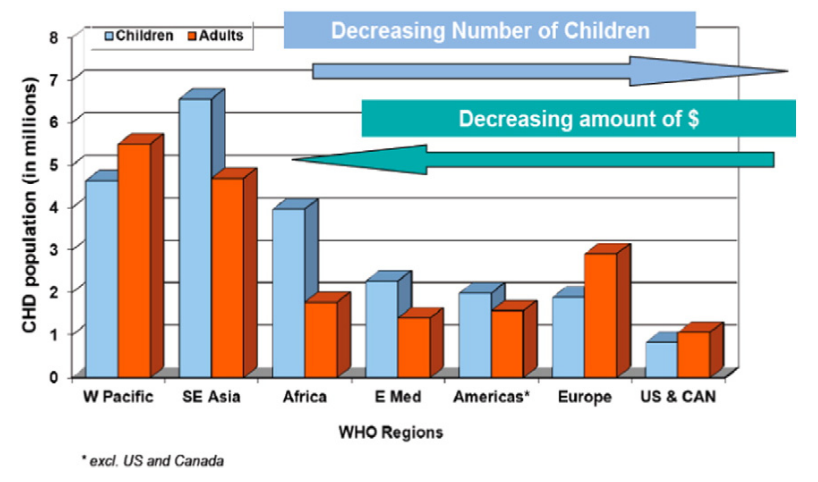
\includegraphics[width=0.7\textwidth]{5/CHD-burden-webb.png}
\caption{Estimated CHD burden in World Health Organization (WHO) regions using incidence rates of approximately 12/1000 and 4/1000 in children and adults, respectively \cite{Webb2015}.}
\label{ch5:fig:CHD-burden}
\end{figure}

%Depending on the cause of the 
The cost of diagnostic techniques and treatment plans impose different levels of financial burden on CHD patients and their families. Certain defects require complex, expensive surgical repairs while others can be treated with less expensive approaches \cite{Mozaffarian2016}. The burden of CHD across the globe was outlined by Webb et al \cite{Webb2015}. Their figure illustrating the prevalence of CHD and the availability of funds with which to treat it can be see in Figure \ref{ch5:fig:CHD-burden}. As the overall mortality of CHD declines, the burden of CHD is expected to increase \cite{Mozaffarian2016}.

% Complications and risks
Unfortunately, the cost of treating CHD is not the only burden a patient must undergo. Patients with CHD are also at increased risk for heart failure and infections \cite{Mozaffarian2016}. Children with CHD are at 19-fold risk for stroke compared to their healthy counterparts \cite{Fox2015}. In a study of Swedish citizens born between 1970 and 1993, Giang et al compared the prevalence of cardiac conditions in patients with and without CHD \cite{Giang2018}. They found that patients who had a CHD diagnosis were at about eight times higher risk for intracerebral hemorrhage and subarachnoid hemorrhage than their non-CHD counterparts. The CHD patients were also more likely to suffer from arrhythmia and heart failure. 

% When are patients diagnosed?
% Expected lifespan
% Treatment plan
% Financial burden

However, cardiac conditions are not the only complications CHD must deal with. Many of these patients also suffer from neurocognitive disorders that co-occur with CHD. Early research in this area focuses on the neurodevelopmental status of neonatal patients pre- and post-surgical intervention. One theory was that some factor or factors in the surgical intervention caused brain injuries in the patients. This idea proved to be inaccurate when researchers began detecting neurological malformations \textit{in utero}.

In a systematic review of available literature regarding prenatal and postnatal presurgical CHD cases and neurodevelopmental outcomes, Mebius et al. identify two theories about the causality of  neurodevelopmental delays and CHD \cite{Mebius2017}. The first theory is that abnormalities in the cardiac system prevent the developing brain from receiving enough oxygen and nutrients, which disrupts prenatal brain development. The second theory is that faulty genetic pathways used during both cardiac and brain development cause both conditions to co-occur. However, 11 articles Mebius et al. found during their review that are related to bloodflow through the umbilical artery suggest a third theory. During the prenatal period, a fetus receives oxygen from the mother via the placenta. If the placenta was not functioning correctly, it could lead to the fetus receiving not enough oxygen. Lower quantities of oxygen throughout prenatal development could potentially cause problems both in brain and cardiac growth. The 11 articles have contradictory results, but some researchers are currently investigating the role of the placenta in CHD and prenatal brain development.

Survival of CHD patients to adulthood has increased from 10\% to 90\% over the last several decades as CHD diagnostic tools and treatments have improved.  Currently, Webb et al. estimate that at least 12 to 34 million adults have CHD, and this number is expected to increase \cite{Webb2015}. The impact of the combination of CHD and neurological conditions throughout a patient's lifetime is starting to be explored. The aging of the CHD population has also sparked interest in the relationships between CHD and adult-stage neurological disorders such as dementia and Alzheimer's. 

While the purpose of this study is not to focus on CHD patients, we chose to use CHD and aging brain images in support of research being performed in the area of relationships between CHD and neurodevelopment.

%To address:
%\begin{itemize}
%\item Common combinations
%\item Joint treatment?
%\item Additional risks?
%\item Joint financial and emotional burden on caretakers? 
%\item CHD, neuro, and aging? Dementia/Alzheimer's? Recent data ... MIND neuroimaging ancillary r01 dec 17
%\end{itemize}


\subsection{Identifying Neurocognitive Disorders}

Neurocognitive disorders are usually diagnosed using at least one of many psychological survey-based evaluations, but these methods are subjective. rs-fMRIs could be used to identify patients who have functional connectivity patterns associated with different neurocognitive disorders, and eventually may be used to identify patients who are at risk for developing these disorders.

\subsubsection{Patient Surveys}

Surveys known to be used for studying the relationship between CHD and neurodevelopment are

\begin{itemize}
\item National Institute of Health Toolbox (3 - 85 years): ``Performance tests of cognitive, motor, and sensory function and self-reported measures of emotional function for adults and children in the general population and those living with a chronic condition''.

\item Sue Beers (4 - 18 years [not inclusive of 18 years]): WASI-II, NEPSY-2, WRAML-2, D-KEFS, WISC-IV, Grooved Pegboard, BRIEF, Beery-Buktenica VMI, ASRS, Conners-3, BASC-II, ABAS-II, PedsQL General, PedsQL Cardiac, Pictoral Scale Self Perception Profile.

\item SVR-III NDT (9 - 13 years [not inclusive of 13 years]): WIAT, NEPSY, WRAML, D-KEFS, WISC-V, Grooved Pegboard, BRIEF, Beery-Buktenica VMI, ASRS, Conners ADHD Index, BASC-II, ABAS-3, PedsQL General, PedsQL Cardiac

\item Bayley Scales of Infant and Toddler Development -III (1 - 24 months): Subtests include cognitive, language, social-emotional, motor, and adaptive behavior tests \cite{Mebius2017}.

\item Battelle Developmental Inventory (Birth - 8 years [not inclusive of 8 years]): Subsets include cognition, communication, social-emotional development, physical development, and adaptive behavior.

\item Developmental Assessment of Young Children (Birth - 6 years [not inclusive of 6 years]): Subtests include cognition, communication, social-emotional development, physical development, and adaptive behavior.

\item Preschool Language Scale + Receptive-Expressive Emergent Language (Birth - 3 years): Total language, auditory comprehension, expressive communication, articulation, receptive language, expressive language, and inventory of vocabulary words.

\item Peabody Developmental Motor Scales (Birth - 5 years): Subtests include reflexes, stationary, locomotion, object manipulation, grasping, visual-motor integration
\end{itemize}

The goal of these surveys is to compare the patient's cognitive function and neurological functions to expected milestones. Certain deviations from certain milestones are indicative of different disorders.

\subsection{Study Cohorts}

The rs-fMRIs used in this study were gathered as part of ongoing studies of the relationship between CHD and neurodevelopment. Data from the CHD/neurodevelopment studies was obtained through studies approved by the IRB at the Children's Hospital of Pittsburgh of UPMC and the University of Pittsburgh. All data is stored and accessed in compliance with HIPPA policies.

The subjects included in this analysis fall into three age groups: neonatal, preadolescent, and fetal. To summarize the cohorts, there were 163 brain rs-fMRIs obtained for the neonatal cohort, 546 brain rs-fMRIs obtained for the preadolescent cohort, and 124 brain rs-fMRIs obtained for the fetal cohort. The fetal cohort also contains 106 rs-fMRIs of the placenta. The race, ethnicity, and gender counts for these three cohorts can be seen in Figures  In the following sections, we describe each cohort in detail. 

\begin{figure}
\centering
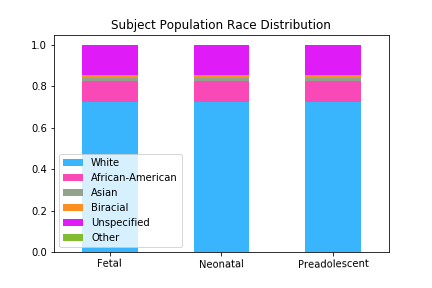
\includegraphics[width=.75\textwidth]{5/demo_clinical_subj_race.png}
\caption{Distribution of subject races for all three cohorts.}
\label{ch5:clinical:race}
\end{figure}%
%
\begin{figure}
\centering
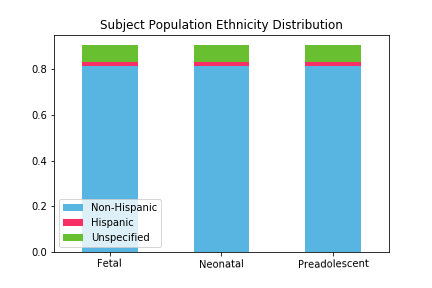
\includegraphics[width=.75\textwidth]{5/demo_clinical_subj_ethnicity.png}
\caption{Distribution of subject ethnicities for all three cohorts.}
\label{ch5:clinical:eth}
\end{figure}

\begin{figure}
\centering
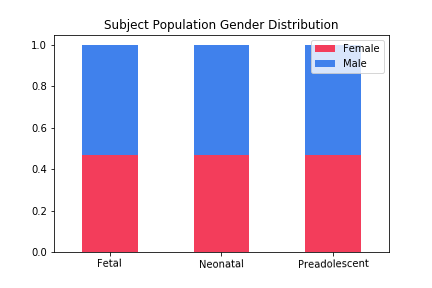
\includegraphics[width=.75\textwidth]{5/demo_clinical_subj_gender.png}
\caption{Distribution of subject genders for all three cohorts.}
\label{ch5:clinical:gender}
\end{figure}

\subsubsection{Neonatal Cohort and Images}

Neonatal subjects have been recruited as part of a prospective observational study. This cohort was scanned at two sites. At Site 1, the subjects were scanned using either a 3T Skyra (Siemans AG, Erlangen, Germany) or a 3T GE . At Site 2, the subjects were scanned using a 3T Philips (*).

The subjects were unsedated during the scans and a ``feed and bundle'' protocol was used to prevent motion during the scans \cite{Windram2011}. The newborns were positioned in the coil to minimize head tilting. Newborns were fitted with earplugs (Quiet Earplugs; Sperian Hearing Protection, San Diego, CA) and neonatal ear muffs (MiniMuffs; Natus, San Carlos, CA). An MR-compatible vital signs monitoring system (Veris, MEDRAD, Inc. Indianola, PA) was used to monitor neonatal vital signs. All scans were performed using a multi-channel head coil. The parameters for the resting-state BOLD MR scans were FOV=240 mm and TE/TR=32/2020 ms with interplane resolution of 4x4 mm, slice thickness of 4 mm, and 4 mm space between slices. The acquired images contained 150 volumes where each volume consisted of 64x64x32 voxels$^3$.

\begin{figure}
\centering
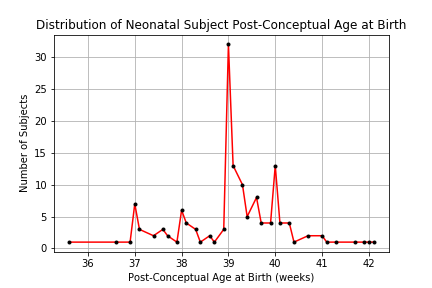
\includegraphics[width=.75\textwidth]{5/demo_neonate_subj_pca.png}
\caption{The distribution of post-conceptual ages at birth of all neonatal subjects.}
\label{ch5:neonates:birthpca}
\end{figure}

\begin{figure}
\centering
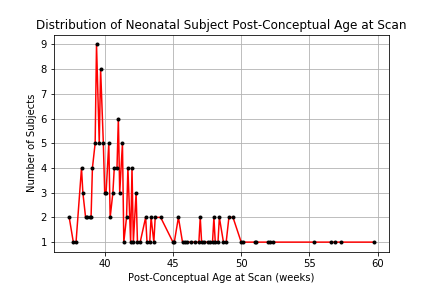
\includegraphics[width=.75\textwidth]{5/demo_neonate_scan_pca.png}
\caption{The distribution of post-conceptual ages at the time of the scan of all neonatal subjects.}
\label{ch5:neonates:scanpca}
\end{figure}

A total of 149 patients were recruited. The average post-conceptual age of the patients at birth was 39.08 weeks and they were on average 42.64 weeks post-conception at the time of the scan. The distribution of post-conceptual ages of the subjects at birth and at the time of the scan can be seen in Figure \ref{ch5:neonates:birthpca} and Figure \ref{ch5:neonates:scanpca}. 

\begin{figure}
\centering
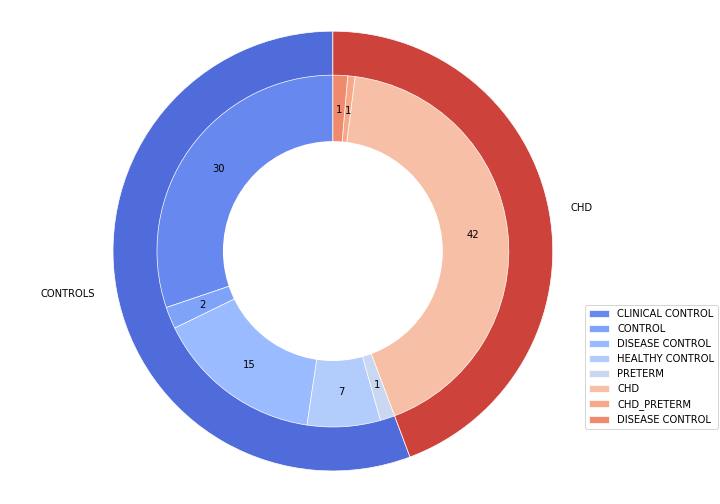
\includegraphics[width=1.0\textwidth]{5/demo_neonate_subj_cohort.png}
\caption{The breakdown of subject groups contained in the Control and CHD neonatal cohorts.}
\label{ch5:neonates:cohorts}
\end{figure}

The subjects were a mix of control subjects and CHD subjects. A comprehensive breakdown description of the subgroups within these two cohorts can be seen in Figure \ref{ch5:neonates:cohorts}. In this figure, the term ``Control'' encompasses both healthy full-term subjects, healthy pre-term subjects, and non-CHD clinical subjects (clinical control and disease control). The CHD group is composed of subjects diagnosed with CHD who were either born full-term or pre-term. Of the entire cohort, 14 subjects underwent two scanning sessions resulting in 163 rs-fMRI scans.

As the neonates were most often asleep during the scan, they exhibit less motion overall compared to our other clinical cohorts. The high-motion neonates are an obvious exception to this concept, but many of the high-motion images contained long periods where the subject was stationary. Applying both the DAG-based framework and the traditional registration framework to these images provided the opportunity to compare the performances of both registration frameworks to each other in the context of the usability gold standard thresholds. 

\subsubsection{Preadolescent Subject Population and Images}

As part of a multicenter study of CHD in preadolescents, we collected rs-fMRIs from nine sites throughout the United States. These images were of patients in the age range of 9 to 13 years who either had CHD or were healthy with no neurocognitive impairments. In addition to the MRI scans, subjects who participated in this study were asked to participate in additional testing  either to determine their neurocognitive outcome status or to perform genetic analyses. % (GET DETAILS FROM NANCY).

\textbf{Preadolescent Cohort.} The multicenter imaging study of preadolescent subjects provides a unique opportunity to evaluate the efficacy of the DAG-based framework on a large subject cohort containing variable amounts of motion. The outcome of this experiment will be used in the next experiment to determine if there are any site-specific or vendor-specific variables influencing patient motion.

%\begin{itemize}
%\item How were the images gathered?
%\item How were the patients recruited?
%\item What are the imaging protocol details?
%\item What other information was collected?
%\end{itemize}

\subsubsection{Fetal Subject Population and Images}

%Real goal is to develop a method of registering fetal brain and placental images so that we can further examine the relationship between placental oxygen levels and fetal brain development. Longitudinally, this technique can be used to determine how placental oxygen flow and fetal brain development impact a patient over the course of his or her life. Once the relationship between the placenta and fetal brain development is better understood, we can determine a set of neuroprotective interventions to employ for at-risk patients before they are born.

Fetal subjects have different constraints on their physical environment than neonates, preadolescents, and adults. As a result, they exhibit unique patterns of motion. The previous subject cohorts discussed in this chapter have the following commonalities: the subject experiences the full effects of gravity, the subject is lying on his back in an MRI scanner, and the subject's head motion is limited by the head coil within the MRI. Any motion in these images is a direct result of the subject himself moving, whether passively (cardiac motion and breathing) or actively (fidgeting or looking around).

A fetal subject is scanned in vivo. He is suspended in amniotic fluid within his mother. The amniotic fluid has buoyancy that reduces the effects of gravity and allows a fetal subject significant freedom of movement. The fetus can rotate, shift, and flip in ways that can only be accomplished when floating in a body of water. The properties of the uterus constrain the physical space in which a motion could occur, but not as much as the head coil and gravity do to the other patient cohorts. A fetus is not guaranteed to be in any specific position at the start of the scan: the scan begins when the mother is ready, not when the fetus achieves a certain pose. 

The fetal subjects underwent fetal echocardiography scans in a cardiac clinic to determine whether they were healthy or had a form of CHD. They were then scanned on an MRI scanner. Images of the fetal brain and the placenta were acquired for each subject. 

We are interested in both the fetal brain and placental images for our work because of the relationship between placenta and brain development. However, these organs have very different physical properties. The fetal brain is a rigid structure floating and moving within the amneotic fluid. It undergoes translation and rotation as a single unit due to passive and active maternal and fetal motions. The placenta, on the other hand, is anchored in place on the uterine wall. It may undergo small translations or rotations due to maternal motion, but it will respond differently to fetal motion. Fetal motions cause nonlinear deformations of the pliable placenta that can only be adequately accounted for using nonlinear registration algorithms. Nonlinear registrations have the potential to deform brain images into physically impossible shapes, so the fetal brain and placenta were manually segmented in their respective images so that each organ could undergo independent motion correction. 

The segmenters were one of a group of four researchers. While one researcher trained the other three group members, the interrater agreement between them is still being determined.

As the fetal subjects have both neurological and placental images, their data will be used to examine the impact of volume registration on different organ types.


%\begin{itemize}
%\item Fetal patients scanned between XX and XX weeks gestational age. 
%\item Imaging protocol details?
%\item What other information is collected about fetus and/or mom?
%\end{itemize}

\subsubsection{Aging Brain Subjects}

The ADNI study was launched in 2003 as a public-private partnership, led by Principal Investigator Michael W. Weiner, MD. The primary goal of ADNI has been to test whether serial magnetic resonance imaging (MRI), positron emission tomography (PET), other biological markers, and clinical and neuropsychological assessment can be combined to measure the progression of mild cognitive impairment (MCI) and early Alzheimer's disease (AD). For up-to-date information, see www.adni-info.org.

%\begin{itemize}
%\item How were the images gathered?
%\item How were the patients recruited?
%\item What are the imaging protocol details?
%\item What other information was collected?
%\end{itemize}

%The second adult cohort comes from the Alzheimer's Disease Neuroimaging Initiative (ADNI) dataset. The ADNI study has been working since 2004 to further Alzheimer's research by gathering, analyzing, and sharing clinical, imaging, genetic, and biochemical biomarkers from the elderly population. The group gathers data from 63 sites in the United States and Canada. During the second phase of the study, sites who have a Philips MRI system gathered resting-state fMRIs from their subjects. This data is freely available to academic researchers through the LONI Image and Data Archive.

The adult cohort encompass many clinical outcomes and a wider age range than the other clinical populations. The adult cohort also allows for another opportunity to study a different type of motion patterns associated with the aging brain rather than the still-developing brain.

\subsection{Summary}
%ELEPHANTS 3-5 sentences about CHD here

While we have amassed a large collection of clinical images, an analysis of purely clinical images is not sufficient in determining which volume registration technique recovers more brain signal. In the next section, we elaborate on this limitation and how we chose to address it.

\section{Simulated Sequences} % ELEPHANTS should this be its own chapter?

There are two major barriers in research surrounding motion correction in rs-fMRIs: gathering data and measuring the effects of the technique. In this section, we elaborate on a simulation designed to address both of these barriers.

\subsection{Background}

Despite the hundreds of images in each of the patient populations described in the previous section, our clinical data would be considered too sparse for ``big data'' analyses. This problem is not unique to our group: it is difficult to obtain enough data from a large number of subjects to perform large-scale studies. Collaborators can band together to create a larger and more diverse data set by participating in multicenter studies. There are some challenges associated with multicenter studies. Each site will have a different scanner, potentially with different field strengths and from different manufacturers. Even ignoring the challenges of harmonizing data obtained using scanners from different companies, each scanner has its own set of unique inhomogeneities in the primary magnetic field. Additional scans of inanimate or human phantoms may be necessary to characterize the differences between all of the scanners involved.

The second barrier to motion correction in rs-fMRI research is the complexity of identifying a gold standard metric to use when evaluating motion correction techniques. The current gold standard metrics developed by Power et al. evaluate motion correction techniques in terms of the reduction of positional differences and signal differences between neighboring volumes. Unfortunately, this approach does not measure the amount of signal recovered or lost though motion correction. A true gold standard evaluation of motion correction would be able to evaluate the BOLD signal present in the image before and after correction. If the BOLD signal prior to patient motion was known, though, there would be no need for image processing in the first place: we would already have the data we are trying to obtain with motion correction.

We address these two barriers by creating a mechanism for generating simulated image sequences. The generated sequences contain simulated brain signal based in areas of the brain associated with resting-state connectivity, scanner noise, and patient motion. Our mechanism can create large quantities of unique image sequences. The simulated image sequences can also serve as a gold standard for evaluating volume registration and motion correction techniques: the signals and noise sources added to the sequence are known with certainty.

%Every MRI scanner is different, even those made by the same manufacturer. To ensure MRI scans obtained from different scanners are comparable.  so a stand-in model for an organ or tissue type is often used to calibrate an MRI scanner. The model is designed to have specific physical properties which mimic the physical properties of the organ or tissue. These properties can be accurately measured during the design process of this model so that the radiologist or researcher looking at images of the model can know the ground truth of the model. Because these models mimic true organs and tissues, they are called phantoms. 

\subsection{SPECTr: Simulated Phantom Emulating Cranial Transformations}

Our mechanism is called Simulated Phantom Emulating Cranial Transformations (SPECTr). A phantom is an object designed to have material properties which mimic those of a specific tissue type or organ. Phantoms, either manufactured objects or healthy humans, are used in multicenter studies to obtain images of the same object or person from multiple scanners. These images are used to harmonize the data taken from the different sites. We call our simulated sequence a phantom because the baseline image itself is known as are the signals added to it to simulate brain activity. 

% ELEPHANTS
When developing the pipeline for SPECTr, it was important to consider the effects of motion and various impacts they have on the BOLD signal. As discussed in CHAPTER, the three effects of motion are positional, spin history, and susceptibility. For simplicity, we combine the spin history and susceptibility effects into ...

\subsection{Materials}

In order to simulate resting-state BOLD signal in an fMRI, two pieces of anatomical information are required. The first is structural information about the brain. The second is the location of functional networks associated with the resting-state BOLD signal.

While it is possible to use clinical images for the structural information, the goal of SPECTr is to be generalizable both for our use and for the use of other researchers. Additionally, clinical images inherently contain some degree of signal from some neuronal processes which could obfuscate the simulated BOLD signal. 

In 1992, the International Consortium for Brain Mapping was formed to develop as set of standards for what is considered a healthy human brain. They used their criteria to develop an initial set of ``average'' brain structural scans based on scans from healthy volunteers. This original set of average brain scans incorporates scans from 305 subjects and is referred to as the MNI305 data. As MRI technology has evolved, the spatial resolution capabilities of the MRI scanners has increased. In 2001, another set of 152 healthy volunteers was recruited to create a higher resolution data set. The scans from the new cohort were linearly registered to the MNI305 data to create the new MNI152 images. % ELEPHANTS citations needed

Herein, we use the MNI152 data set as available at the website for the McConnell Brain Imaging Centre at McGill University. This data set contains five images: a T1-weighted scan, a T2-weighted scan, a proton density weighted scan, and two binary masks for the head and the brain. Each of the structural scans was designed to highlight the properties of different tissues in and around the brain. Proton density scans were developed for the purpose of detecting blood-related signal. As BOLD images essentially perform the same purpose over a period of minutes, we choose to use the proton density weighted scan as the structural base for the simulated images. % ELEPHANTS citations needed

The functional network information is more difficult to find than structural atlases. The Functional Imaging in Neuropsychiatric Disorders Lab at Stanford has developed two sets of functional atlases. The atlases are divided into regions of interest (ROIs) associated with individual networks. The first set of atlases contains 90 functional ROIs which compose 14 networks. The second set of atlases contains 499 functional ROIs and has more gray matter coverage. For simplicity, we chose to use the original ROIs associated with the dorsal and ventral default mode networks.

\subsection{Simulation Pipeline}

\subsubsection{Baseline Sequence}

\begin{figure}
\centering

\includegraphics[width=.5\textwidth]{5/pipeline.png}
\caption{An overview of the SPECTr simulation pipeline. Using atlas data, a simulated phantom containing brain signal, scanner noise, and patient motion is generated.}
\label{ch5:spectr_flow}
\end{figure}

The process for generating a simulated sequence using the data discussed in the previous section has several steps. An overview of the pipeline can be seen in Figure \ref{ch5:spectr_flow} We cover these steps in detail in this section.

The MNI152 proton density image is a whole head image. To remove the skull, we apply the brain mask to the proton density weighted image. The resulting image contains only brain tissue.

The spatial resolution of the structural brain image is 1 mm$^3$. The spatial resolution for a single volume in a rs-fMRI sequence is less granular at 4mm$^3$. To achieve this resolution, the structural volume must be downsampled. After the downsampling, the size of the structural image is reduced from 181x217x181 voxels to XXxXXxXX voxels. %ELEPHANTS interpolation?

Now that the structural image is the correct spatial resolution, it must be replicated to create the temporal sequence. Part of this step includes creating a new dimension in the data. The affine matrix which represents the resolution of the image has the following structure:

\begin{equation}
\begin{bmatrix}
 r_x &  0   &  0   & c_x\\ 
 0   &  r_y &  0   & c_y \\ 
 0   &  0   &  r_z & c_z \\ 
 0   &  0   &  0   & 1 
\end{bmatrix}
\end{equation}

\noindent where $r_x, r_y,$ and $r_z$ represent the spatial resolution in the $x, y,$ and $z$ axes, respectively and $c_x, c_y,$ and $c_z$ represent the location of the origin in voxels. To convert the image from a 3D volume to a 4D sequence, we add a row and a column to this matrix so that it now has the structure:

\begin{equation}
\begin{bmatrix}
 r_x &  0   &  0   & 0 & c_x\\ 
 0   &  r_y &  0   & 0 & c_y \\ 
 0   &  0   &  r_z & 0 & c_z \\ 
 0   &  0   &  0   & t & 0 \\
 0   &  0   &  0   & 0 & 1 
\end{bmatrix}
\end{equation}

\noindent where $t$ is the desired temporal resolution. We choose a temporal resolution of 2 seconds for our simulated sequence. The downsampled image volume is replicated and concatenated along the new temporal dimension to create a sequence that is 150 image volumes long. This sequence is referred to as the base phantom sequence as it contains no brain signal, noise, or motion.

\subsubsection{Brain Signal}

The next step in the pipeline is to add BOLD signal to the sequence. % ELEPHANTS (Why brain signal next?) 
We combine the functional ROIs from the dorsal and ventral default mode networks into a single binary functional ROI image. This image is referred to as the default mode network (DMN) mask. 

For each nonzero voxel in the DMN mask, a temporal signal is generated. We chose to model the BOLD response as a cosine signal following the formula

\begin{equation}
s(\vec{v}, t) = a*(cos(f_0 * (t-t_{shift})) - a_shift).
\label{ch5:bold_eq}
\end{equation}

\noindent This equation is for a scaled cosine function with both temporal and amplitude shifts. The temporal and amplitude shifts, $t_{shift}$ and $a_{shift}$ respectively, are randomly generated for each voxel from uniform distributions. Once chosen, they are consistent across the voxel's generated temporal signal. The other parameters, $a$ and $f_0$, were specified using existing research. 

In 2007, Biswal et al. performed a study evaluating methods to reduce changes in the BOLD signal not directly related to brain activity (i.e., vascularity). They identified a low-frequency spectral amplitude of 0.04 Hz as the highest frequency related to BOLD signal consistent not only through scans of individual patients but in group-wise analyses. Based on their work, we chose the fundamental frequency $f_0$ to be 0.04 Hz. % ELEPHANTS citation

The scaling factor $a$ was chosen based on Power et al.'s usability criteria. As they state that any signal change between volumes above 2.5\% of the maximum voxel value is unlikely to be due to brain activity, we used an amplitude of 20 units on a scaled voxel value range of [0, 1000]. % ELEPHANTS citation

The generated BOLD signals were added to the baseline image sequence, but were also saved in a separate image sequence file for reference during analysis. The generated sequence with only BOLD signal is referred to as the brain signal sequence.

\subsubsection{Scanner Noise}

The next step in the pipeline is to add scanner noise to the brain signal sequence. In a regular rs-fMRI of a patient, the noise in the sequence is the result of two factors: the spin history effects of motion and the susceptibility effects of motion. To simplify the simulation, we choose to model the resulting noise rather than the individual sources.

Signal acquired by MRI scanners is first recorded as a raw data matrix in k-space. K-space contains spatial frequency information. The coordinate system of k-space differs from the coordinate system of physical space. In k-space, the closer a point is to the center of a zero-centered data matrix, the lower its frequency or phase. The brighter a point in the raw data matrix is, the larger its magnitude. 

While frequency is a continuous spectrum, data is usually divided into low frequency data and high frequency data. Low frequency data in imaging is areas of an image where the pixel or voxel values slowly. In physical space, these areas are the smooth areas that contain content. In Figure REF, the skin on the woman's face would be considered low frequency data. High frequency data represents the areas in an image where the pixel or voxel values change rapidly in a small area. Areas with many edges in them contain higher frequency data. In Figure REF, the feather in the woman's hat would be considered high frequency data. % Need a figure ELEPHANTS 

Generally speaking, images contain more low frequency information than high frequency information. We wish to be able to control the amount of noise added to each component independently, so we choose to add noise to the sequence in k-space.

When adding scanner noise to the brain signal sequence, we add noise to each image volume independently. The image volume is transformed from physical space into k-space using the fast Fourier transform (FFT). To force the image to be zero-centered, we perform a FFT shift on the Fourier space data. A matrix the same size and shape as the image volume is created. The matrix is then filled with complex Gaussian noise, $n(\vec{l})$ where

\begin{equation}
|n(\vec{l})| = w_m * r_m, r_m~N(0,1)
\end{equation}

\noindent and

\begin{equation}
\angle n(\vec{l}) = w_p * r_p, r_p~N(0,1)
\end{equation}

\noindent In these two equation, $\vec{l}$ is the location of the point in the matrix, $w_*$ represents the weight assigned to the component, $r_*$ represents the noise random variable independently generated from a standard normal distribution, and the subscripts $m$ and $p$ refer to the magnitude and phase components, respectively. The complex noise is weighted so that the magnitude of the noise has a greater contribution than the phase of the noise, that is $w_m > w_p$ 

The matrix of complex noise is added to the zero-centered k-space image volume. The noisy k-space volume is unshifted and undergoes an inverse Fourier transform to change the data back to physical space.

\subsubsection{Patient Movement}

Now that the ground truth brain orientation and BOLD signal have been established, patient motion can be added to the BOLD phantom sequence. One of the aims of this document is to establish that patients from different populations exhibit different motion patterns. As we have not yet established what those motion patterns are, we developed a generic motion model for the simulation.

During an rs-fMRI scan, a patient theoretically has the freedom to rotate his head around three different axes, translate his head along three different axes, or some combination of translations and rotations. Realistically, once a patient has settled in the scanner, it becomes difficult for his head to only undergo translation. It is more likely that he will rotate his head. For the simplicity of the simulation, we assume no head translations occur during the scan.

A rotational transformation can be represented as a matrix. Rotations about a single axis are represented as followed:

\begin{equation}
R_x(\alpha) = \begin{bmatrix}
 1 &  0          & 0     \\ 
 0 &  cos\alpha  & sin\alpha \\ 
 0 &  -sin\alpha & cos\alpha \\ 
\end{bmatrix}
\end{equation}
\begin{equation}
R_y(\beta) = \begin{bmatrix}
 cos\beta &  0 & -sin\beta \\ 
 0        &  1 & 0         \\ 
 sin\beta &  0 & cos\beta  \\ 
\end{bmatrix}
\end{equation}
\begin{equation}
R_z(\gamma) = \begin{bmatrix}
 cos\gamma  & sin\gamma  & 0 \\ 
 -sin\gamma & cos\gamma  & 0 \\ 
 0          & 0          & 1 \\ 
\end{bmatrix}
\end{equation}

Rotational transforms are applied to the origin of the image. However, the origin of the image is not necessary anatomically significant. Head motion naturally occurs about the base of the neck. We can approximate the location of the base of the neck by calculating the center of mass of the brain. First, the image volume is thresholded to separate the brain from the background. Then the locations of the ``on'' voxels are averaged to calculate the center of mass. 

Motion is added to the noisy image sequence one volume at a time. No motion is applied to the first volume in the sequence, but volume is used to calculate the center of mass of the brain. For each subsequent volume, the angles of rotation about the x-, y-, and z-axes are each randomly generated from a standard normal distribution to create rotational change matrices, $R_{*,\Delta}$ (where the subscript $*$ represents $x$, $y$, or $z$). The new rotations $R_{*,\Delta}$ are added to the rotations from the previous step $R_{*,i-1}$ to create the rotation matrices for the current volume, $R_{*,i}$:

\begin{equation}
R_{*,i} = R_{*,i-1} + R_{*,\Delta}
\end{equation}

The three rotational transformations are combined into one matrix via multiplication: 

\begin{equation}
R_i = R_{x, i}(\alpha) R_{y,i}(\beta) R_{z,i}(\gamma)
\end{equation}

The compound transformation $R_i$ is then applied to the image at the center of mass calculated from the original image volume. \textit{Note: Since the simulation is constrained by the assumption of no head translations, the center of mass will remain consistent throughout the image sequence.}

After motion has been added to every image volume in the sequence, the sequence with motion is ready to be used in motion correction analyses.

\subsection{Implementation}

SPECTr is implemented in Python (version 3.7.3). The \lstinline{nipy} library (version 0.4.1) was used to load images, save images, and combine the functional ROIs. The \lstinline{numpy} library (version 1.17.4) was used for matrix manipulations involved in the brain signal and noise generation steps. The image processing library \lstinline{skimage} (version 0.14.2) was used to calculate the center of mass. The Python wrapper \lstinline{SimpleITK} (version 1.2.4) of the Insight Toolkit library for image analysis was used to perform the rotational transformations associated with patient motion.

The source code for SPECTr is available on Github at \url{https://github.com/jmschabdach/SPECTr}.


%First, a reasonable range of head rotation about the x-, y-, and z-axes was established. These angle ranges are used to generate rotational transformation matrices for $N-1$ image volumes. The transformations are applied to each image volume after the first volume in the BOLD phantom sequence. The transformed image sequence is referred to as the BOLD phantom sequence with motion and the rotational transformation matrices are saved as the ground truth for the transformations between each image volume and the template volume. 
%The BOLD phantom sequence serves as the ground truth for any motion correction pipeline: it contains the known brain orientation and BOLD signal independent from head motion and scanner noise.

\subsection{Experiments Involving Simulated Images}

We generated 90 image sequences from the MNI152 proton density image and the default mode network functional ROIs using the process described in the previous section. The image sequences were divided into three groups with different degrees of scanner noise. All simulated images underwent both registration techniques described in Chapter \ref{ch:mri}. The registered images also underwent independent component analysis (ICA) using FSL's MELODIC (Multivariate Exploratory Linear Optimized Decomposition into Independent Components) tool. % ELEPHANTS SOURCES

The registered images will undergo the same type of analysis as the clinical images. The ICA technique will be used to determine how much brain signal was recovered by each registration technique.

This particular experiment will be one of the first to investigate how much true BOLD signal is preserved through motion correction. One of the major drawbacks to existing motion correction pipelines is that they remove signal along with noise. In clinical data, there is no way to know the ground truth signal contained within the image; however, simulated phantom images have a de facto known ground truth signal. The design for this experiment can be used to evaluate how much BOLD signal is recovered by other motion correction pipelines, and how close the recovered signal is to the signal of interest.

\section{Summary}

In this chapter, we discussed our three major data sets, which are drawn from simulated data, pediatric data, and aging brain data. The simulated data were generated using a rs-fMRI simulation pipeline developed in-house and were used for the purpose of measuring ground truth signal recovered by motion correction techniques. The pediatric data were obtained through prospective studies of CHD and neurodevelopment being conducted at the UPMC Children's Hospital of Pittsburgh. The pediatric and aging brain images were used to compare the two volume registration techniques in a standalone analysis as well as in the context of a motion correction pipeline. We also used these images to examine patterns of motion unique to different age groups. 
\chapter{METHODS}

\section{Volume Registration and Motion Correction}

\section{Pattern Detection}

\section{Tools}

Cite nipypy, ANTs, FSL, etc. here

\section{Metrics and Analyses}

Power et al. thresholds

Correlation ratio matrix

Statistical tests

Dice coefficients?
%\chapter{PRELIMINARY RESULTS}
\label{ch:results}

\section{Comparison of Volume Registration Methods}

\subsection{Subject Position Variability in the Registered Images}

\begin{table}[t]
\centering
\caption{The mean and standard deviation for each sequence’s correlation ratio matrix for every subject.}
\label{tab:crm-stats}
\begin{tabular}{|c|c|c|c|c|c|c|}
\hline
\multicolumn{1}{|l|}{\textbf{}} & \multicolumn{2}{c|}{\textbf{Original Sequence}}                                        & \multicolumn{2}{c|}{\textbf{Traditional Registration}}                                 & \multicolumn{2}{c|}{\textbf{DAG-based Registration}}                                   \\ \hline
\textbf{Subject}                & \textbf{Mean} & \textbf{\begin{tabular}[c]{@{}c@{}}Standard \\ Deviation\end{tabular}} & \textbf{Mean} & \textbf{\begin{tabular}[c]{@{}c@{}}Standard \\ Deviation\end{tabular}} & \textbf{Mean} & \textbf{\begin{tabular}[c]{@{}c@{}}Standard \\ Deviation\end{tabular}} \\ \hline
0                               & 0.04476       & 0.02707                                                                & 0.03842       & 0.01167                                                                & 0.03194       & 0.01082                                                                \\ \hline
1                               & 0.04339       & 0.02926                                                                & 0.03323       & 0.00771                                                                & 0.03903       & 0.01315                                                                \\ \hline
2                               & 0.03464       & 0.01773                                                                & 0.04522       & 0.01359                                                                & 0.03768       & 0.00775                                                                \\ \hline
3                               & 0.03431       & 0.00264                                                                & 0.03203       & 0.01097                                                                & 0.03528       & 0.00289                                                                \\ \hline
4                               & 0.03288       & 0.00462                                                                & 0.02601       & 0.00981                                                                & 0.03364       & 0.00514                                                                \\ \hline
5                               & 0.03234       & 0.01376                                                                & 0.02986       & 0.00958                                                                & 0.03390       & 0.00800                                                                \\ \hline
6                               & 0.03145       & 0.00730                                                                & 0.02691       & 0.00685                                                                & 0.03065       & 0.00496                                                                \\ \hline
7                               & 0.02970       & 0.03314                                                                & 0.03331       & 0.00736                                                                & 0.03025       & 0.00969                                                                \\ \hline
8                               & 0.02728       & 0.01044                                                                & 0.03060       & 0.00500                                                                & 0.03359       & 0.00791                                                                \\ \hline
9                               & 0.02467       & 0.00305                                                                & 0.03354       & 0.00513                                                                & 0.02467       & 0.00303                                                                \\ \hline
10                              & 0.02446       & 0.00163                                                                & 0.03535       & 0.00293                                                                & 0.02446       & 0.00163                                                                \\ \hline
11                              & 0.02422       & 0.01161                                                                & 0.02958       & 0.00559                                                                & 0.02617       & 0.00981                                                                \\ \hline
12                              & 0.02338       & 0.00060                                                                & 0.02467       & 0.00304                                                                & 0.02338       & 0.00060                                                                \\ \hline
13                              & 0.02280       & 0.00101                                                                & 0.02447       & 0.00163                                                                & 0.02279       & 0.00101                                                                \\ \hline
14                              & 0.01968       & 0.01040                                                                & 0.02338       & 0.00060                                                                & 0.02740       & 0.00664                                                                \\ \hline
15                              & 0.01942       & 0.00526                                                                & 0.02279       & 0.00101                                                                & 0.02939       & 0.00548                                                                \\ \hline
16                              & 0.01414       & 0.00133                                                                & 0.01512       & 0.00178                                                                & 0.01520       & 0.00184                                                                \\ \hline
\end{tabular}
\end{table}

Each rs-fMRI sequence in the cohort underwent registration using both frameworks. For each sequence, the correlation ratio between every possible pair of volumes was calculated. A set of metrics of the correlation ratio matrices for each sequence can be seen in Table \ref{tab:crm-stats}. This table shows that the original sequences generally have higher average correlation ratios and contain more variation in their correlation ratios than the globally registered images. The registration methods were able to reduce the mean and variability of the correlation ratios across all subjects in the cohort who had original correlation ratio averages of at least 0.035.

\subsection{Comparison of Motion Correction Methods}

%\begin{figure}[th]
%\centering
%\includegraphics[width=1.0\textwidth]{figures/histograms-both.png}
%\caption{Histograms of the FD and DVARS values between all pairs of neighboring image volumes for the DAG-based registration (solid) and the traditional correction (dotted). The vertical red line in each histogram indicates the threshold of acceptance for that metric. The DAG-based registration method’s histograms are distributed closer to the threshold for each criteria than the traditional registrations method’s.}
%\label{fig:hists}
%\end{figure}

\begin{table}[th]
\centering
\caption{The mean, median, standard deviation, skewness, and kurtosis of the histograms of FD and DVARS values for all image types were calculated. The histograms for the DAG-based method have lower means, medians, and standard deviations than those of the first volume correction method.}
\label{tab:hists}
\begin{tabular}{|l|c|c|c|c|c|c|}
\hline
                                    & \multicolumn{3}{c|}{\textbf{FD Values (mm)}}                                                                                         & \multicolumn{3}{c|}{\textbf{DVARS Values (units)}}                                                                                   \\ \hline
\textbf{Statistic}    & \multicolumn{1}{l|}{\textbf{None}}         & \multicolumn{1}{l|}{\textbf{Traditional}}  & \multicolumn{1}{l|}{\textbf{DAG-based}}    & \multicolumn{1}{l|}{\textbf{None}}         & \multicolumn{1}{l|}{\textbf{Traditional}}  & \multicolumn{1}{l|}{\textbf{DAG-based}}    \\ \hline
Mean                                & 1.07                                       & 2.18                                       & 1.22                                       & 63.14                                      & 135.15                                     & 97.23                                      \\ \hline
Median                              & 0.30                                       & 1.46                                       & 0.56                                       & 35.19                                      & 133.48                                     & 77.75                                      \\ \hline
Standard Deviation                  & 1.97                                       & 2.35                                       & 1.61                                       & 70.00                                      & 83.48                                      & 77.14                                      \\ \hline
Skewness (-)                        & 3.86                                       & 3.08                                       & 3.00                                       & 2.76                                       & 1.13                                       & 1.55                                       \\ \hline
Kurtosis (-)                        & 23.29                                      & 17.74                                      & 17.12                                      & 14.28                                      & 7.79                                       & 7.44                                       \\ \hline
\end{tabular}
\end{table}

\begin{table}[th]
\centering
\caption{The number of frames recovered by each global volume registration framework for each threshold.}
\label{tab:thresholds}
\begin{tabular}{|l|r|r|r|}
\hline
\textbf{Threshold} & \textbf{None} & \textbf{Traditional} & \textbf{DAG-based} \\ \hline
FD (0.2 mm)        & 966           & 175                  & 569                \\ \hline
DVARS (25 units)   & 781           & 78                   & 297                \\ \hline
Both               & 619           & 61                   & 258                \\ \hline
Both (\%)          & 24.27\%       & 2.39\%               & 10.11\%            \\ \hline
\end{tabular}
\end{table}


The FD and DVARS values were calculated to determine how many volumes in each registered sequence met the FD and DVARS thresholds. The FD and DVARS values also considered to be distribution functions representing the effects of no registration, traditional registration, and DAG-based registration. These distributions were compared using the Kolmogorov-Smirnov test, which compares the empirical distribution functions of two samples. There were statistically significant differences between the FD and DVARS values of all sequences at $p < 2.2*10^{-16}$. Statistics calculated for the FD and DVARS value histograms of both motion correction methods can be seen in Table \ref{tab:hists}.

Power et al.'s usability thresholds were used to determine how many volumes were recovered by each framework \cite{Power2014}. Table \ref{tab:thresholds} shows the number of volumes meeting each threshold, with the traditional and DAG-based frameworks recovering 2\% and 10\% of volumes, respectively. These results show that the DAG-based registration technique produces sequences with lower FD and DVARS value than the traditional global registration method does.

%\chapter{DISCUSSION}
\label{ch:discussion}

\section{Comparison of Volume Registration Methods}

Resting-state BOLD MR images are used to evaluate the functional architecture of a patient’s brain . Because resting-state BOLD images are highly susceptible to motion, development of strong post-acquisition motion correction techniques is vital. Current pipelines for mitigating motion after sequence acquisition vary in terms of efficacy and effectiveness, but all begin with global volume registration. In this study, we compared the corrective performance of two global volume registration methods, the traditional framework and a novel DAG-based framework, on a set of 17 neonatal rs-fMRIs. 

The correlation ratio matrices, FD, and DVARS values were calculated for each sequence. The decrease in the mean and standard deviations of the correlation ratio matrices for the registered sequences indicate that global volume registration reduces some effects of motion in rs-fMRIs. The histograms of the FD and DVARS values in the registered sequences show that the DAG-based method was better able to correct volumes to meet Power et al’s thresholds than the traditional registration method. These results indicate that the DAG-based global registration method is better able to reduce the effects of motion than the traditional global registration method when correcting motion in neonatal images. While no entire sequences were recovered, some high-motion volumes within each sequence were recovered by the DAG-based registration method that were not recovered by the traditional registration method. 

\subsection{Relation to Existing Work}
To the best of our knowledge, the only other study that has used a variant of the DAG-based method was performed by Liao et al \cite{Liao2016}. Liao et al’s dataset consisted of 10 fetal rs-fMRIs. In each of these sequences, the fetal brain, fetal liver, and placenta were manually segmented in the first volume of the sequence as well as in five other randomly chosen volumes. These overlap of these manual segmentations before and after registration as measured using the Dice coefficient was used to quantify the amount of motion in each sequence. Even though the Dice coefficients increase more in each sequence after Liao et al.’s registration than after traditional registration, their measure of positional change fails to quantify any changes in position between any other pairs of volumes that do not have manual segmentations. 

\subsection{Limitations and Future Work}

Subject motion during rs-MRI scans affects both the recorded position and orientation of the subject as well as the established magnetic spin gradients within the skull. The DAG-based technique can correct the positional effects of motion, but it cannot correct the effects of the motion that disrupt the magnetic spin gradients. Methods for prospectively estimating subject motion exist and can be used to change slice positions in each volume during acquisition. Retrospective techniques to correct for this effect will require shot-to-shot modeling of macroscopic $B_0$ fields and are beyond the scope of the present research.

In the future, we plan to apply the DAG-based technique to a cohort of preadolescent images for the purpose of characterizing motion in a large cohort as well as to a cohort of neonatal images to address the problem of correcting motion of multiple organs in images with large amounts of motion.  

\subsection{Conclusions}

In this feasibility study, we applied two global registration methods to set of rs-fMRIs of 17 healthy neonates. We showed that both global registration techniques reduce the amount of motion in the images as measured using the correlation ratio. We then showed that the DAG-based framework is better at correcting images to a pair of established gold standard thresholds for resting-state BOLD MRI usability than the traditional framework. In the future we plan to apply the DAG-based framework to other patient populations and multi-organ problems.
%\chapter{Conclusions}
This is the second chapter of the present dissertation. It is more interesting than the first one, for it is the last one.


%
%\appendix                          After this command, chapters will be formatted as appendices. For example:
%\chapter{Raw data}
%
\safebibliography{sources}          
%\safebibliography is used the same way as \bibliography, but gives pittetd a greater chance to succeed in formatting the bibliography when non-standard BibTeX styles are used.
\end{document}
